\subsection{Functional failure study}
\label{sec:failure-case-study}

% What is done here, introduction
In this section, a practical case of functional failure of an integrated function is studied.
It was found on the real product described previously in \ref{sec:real-product-study}.
exploring robustness when reducing the amount of external protection devices.

Failure in cascade of the regulation function, when the disturbance propagates through all blocks

%TODO: Investigate on source of failure ?
Single block, multiple block, multiple nets, etc.

%TODO: Review
In case of failure, the primary supply can cause the entire product to shut down.
Indeed, this entire system requires soft-start behavior to avoid generating harmful voltage spikes to powered functions.
This functionnality enforces the system to start on a \br{long} period of time, in the order of a hundred microseconds.

When the system is stressed with an \gls{esd}, voltages and currents are fluctuating inside the block.
Under certain conditions, and especially important stress levels, the block will detects some nodes going in undervoltage or overvoltage.
This will cause the block to go into safe or protected mode, where it will restart because the functionnality cannot be assured properly.
The direct consequence is that the block will require again a hundred microseconds to be again in normal operation mode.

This failure can in a first time be observed in simulation.
An \gls{ESD} is superimposed on the DC battery voltage.
This is the most likely entry point for a stress, because the \gls{IC} exposes a pin to the external workd and is usally connected to the battery via a long cable
To detect is a block reset happened, the voltage on the first voltage regulator is observed.
Fig. \ref{fig:wvf-vboost} shows the stress waveform on the input.

\begin{figure}[!htbp]
  \centering
  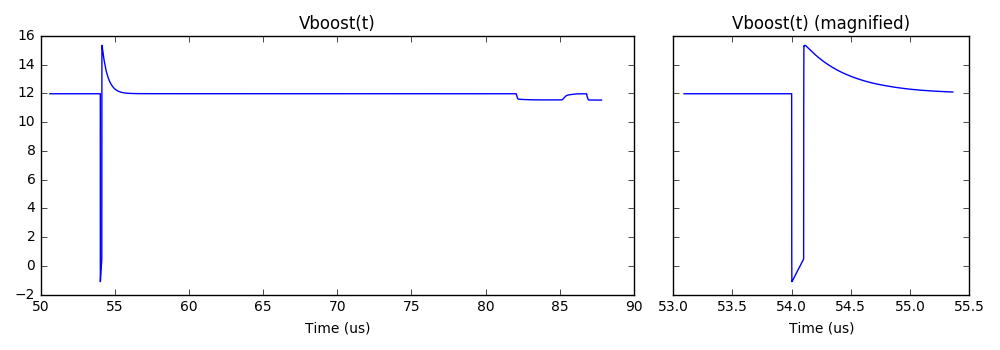
\includegraphics[width=0.9\textwidth]{src/3/figures/vboost.png}
  \caption{Waveform of the vboost input pin}
  \label{fig:wvf-vboost}
\end{figure}

Fig. X shows a simulation where a small glitch can be observed on the regulated output, but without clear reset or soft-failure signature.
In this case, the block and the rest of the product is most likely not affected by the ESD.

WAVEFORM OUTPUT NO RESET

Fig. \ref{fig:wvf-v2p5} shows a simulation where a clear reset hapened.
The output voltage is maintained by a 100nF capacitor.
However, it clearly goes down after the \gls{esd} and rises slowly afterward, a sign that the block went into full reset and restard.

\begin{figure}[!htbp]
  \centering
  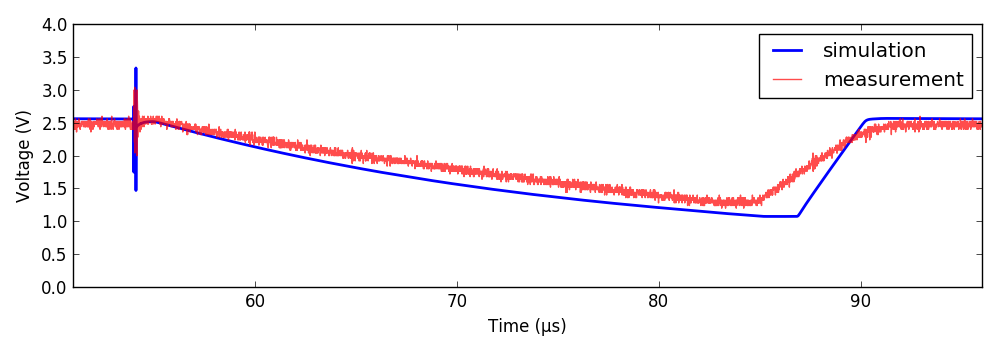
\includegraphics[width=0.9\textwidth]{src/3/figures/v2p5.png}
  \caption{Waveform of the v2p5 output pin}
  \label{fig:wvf-v2p5}
\end{figure}

By going inside the \gls{IC}...

bandgap, voltage ref, current ref, etc

\begin{figure}[!htbp]
  \centering
  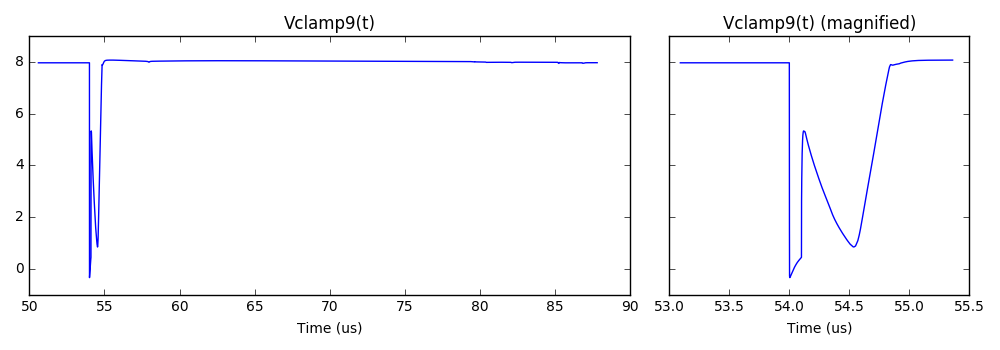
\includegraphics[width=0.9\textwidth]{src/3/figures/vclamp9.png}
  \caption{Waveform of the vclamp9 internal net}
  \label{fig:wvf-vclamp9}
\end{figure}

\begin{figure}[!htbp]
  \centering
  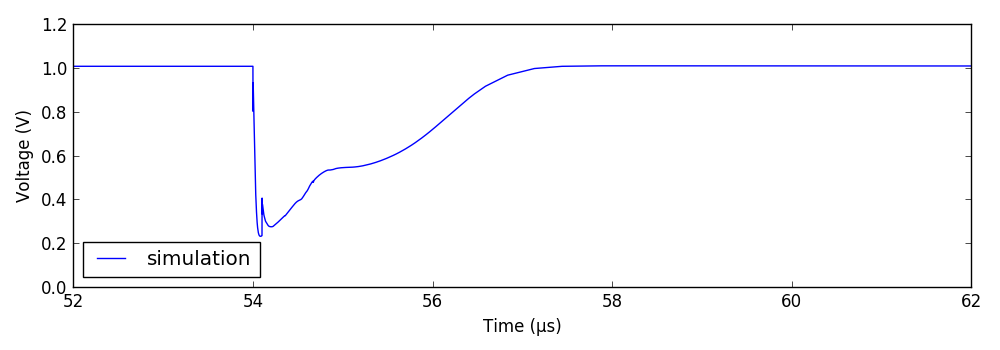
\includegraphics[width=0.9\textwidth]{src/3/figures/v1p0.png}
  \caption{Waveform of the vref1p0 internal net}
  \label{fig:wvf-v1p0}
\end{figure}

DISCUSSION AROUND INCREASE OF FAILURE LENGTH after each stage of the chain

WHICH SIGNAL IS GOING out of spec first ?
